\chapter{Partitions}
A first course in combinatorics typically focuses on two types of partitions: set partitions and integer partitions. We will begin with a brief discussion of set partitions, followed by a more in-depth exploration of integer partitions. 
\section{Set Partitions}
Notice how there are $6$ ways to partition the set $\{1,2,3,4\}$ into $3$ blocks. These are,
    \begin{enumerate}
        \item $[1],[2],[3,4]$
        \item $[1],[2,3],[4]$
        \item $[1,2],[3],[4]$
        \item $[1,4],[2],[3]$
        \item $[1,3],[2],[4]$
        \item $[2,4],[1],[3]$
    \end{enumerate}
This kind of counting is generalized by what are called a Stirling numbers of the $\nth{2}$ kind. More formally,
\begin{definition}
A set partition of a finite set $B$ into $k$ ``blocks'' is a collection of $k$ subsets of $B$ say $B_1,\cdots,B_k$ such that 
\begin{enumerate}
    \item $\bigcup_{i=1}^kB_i = B$,
    \item $B_i\cap B_j=\emptyset$ for all $i\neq j$,
    \item and none of the $B_i$'s are empty. 
\end{enumerate}
\end{definition}
\begin{definition}
If $B=[n]=\{1,\cdots,n\}$ then a Stirling number of the $\nth{2}$ kind $S(n,k)$, is the number of set partitions of $B$ into $k$ blocks.
\label{d:Str2}
\end{definition}
We take $S(0,0)$ to be $1$ by convention. Additionally, the fact that $S(n,n)=1$, $S(n,0)=0$, and $S(n,1)=1$ follow immediately. Per usual we state a few identities concerning these numbers.
\begin{claim}
For all $n,k\geq 0$, with $n\geq k$ we have $S(n,k)=S(n-1,k-1)+kS(n-1,k)$
\end{claim}
\begin{proof}
By the \cref{d:Str2}, the L.H.S of our claim counts the set of partitions of $[n]$ into $k$ blocks. 
We give a double-counting argument; 
one, the partitions where $n$ is itself a block, two, the partitions where the block containing $n$ has a size of at least two. To count the partitions where $n$ is a block by itself, we can take $n$ out, choose a partition of $[n-1]$ into $k-1$ blocks in $(n-1,k-1)$ ways, and enlarge the chosen partition to obtain a partition of $[n]$ into $k$ blocks by adding $\{n\}$ as the $n$-th block. To count the partitions where the block containing $n$ has a size at least two, choose a partition of $[n-1]$ into $k$ blocks in $S(n-1 1,k)$ different ways, and for each of such choices create a partition of $[n]$ into $k$ blocks in $k$ different ways by placing $n$ inside one of the $k$ blocks. Putting all together, we see that the number of partitions of $[n]$ into $k$ blocks is $S(n-1, k-1)+kS(n-1, k)$, as required.
\end{proof}
\begin{claim}
    $S(n,2)=2^{n-1}-1$
\end{claim}
\begin{proof}
Each partition of $[n]$ into
two blocks, say $\{B_1, B_2\}$, can be constructed by first choosing the subset $B_1$ in $2^n-2$ ways (since $B_1$ cannot be neither empty nor the whole set $[n]$), which forces
$B_2$ to be equal to  $[n] \backslash B_1$. Next, we divide our number of choices, $2^n - 2$, by $2$ to account
for the fact that the order of the blocks inside the partition is irrelevant to see why the claim is true. 
\end{proof}
\begin{claim}
    $S(n,n-1)=\binom{n}{2}$
\end{claim}
\begin{proof}
Each partition of $[n]$ into $n-1$ blocks must contain exactly one block of size $2$, which completely determines the rest of the blocks, namely the remaining $n-2$ blocks of size $1$. Therefore the set of partitions of $[n]$ into two blocks is in bijection with the set of $2$ element subsets of $[n]$. Now the claim follows.
\end{proof}
\begin{claim}
    \[
    S(n,k) = \dfrac{1}{k!}\sum_{j=0}^{k}(-1)^{k-j}\binom{k}{j}j^n
    \]
\end{claim}
\begin{proof}
To count the number of surjective functions $f: [n] \to [k]$, we can first fix a set partition $\{B_1,\ldots,B_k\}$ of $[n]$ into $k$ blocks in $S(n,k)$ ways, then make a linear arrangement $w_1 w_2 \cdots w_k$ with the elements of $[k]$ in $k!$ ways, and then finally the set $f^{-1}(w_i) = B_i$ to see why there are $S(n, k)k!$ choices of $f$. By the virtue of \cref{c:SurjMap} we are done.
\end{proof}
\begin{definition}[Bell Numbers]
The number of all partitions of $[n]$ is called a bell number and is denoted by $B(n)$. More specifically,
\[
B(n) = \sum_{k=1}^nS(n,k)
\]
\label{d:BellN}
\end{definition}
We are interested in coming up with a recurrence of $B(n)$ which is independent of any $S(n,k)$s. 
\begin{claim}
    \[
    B(n+1) = \sum_{k=0}^{n}\binom{n}{n-k}B(k)
    \]
\end{claim}
\begin{proof}
By \cref{d:BellN}, the L.H.S of our claim counts the set of partitions of $[n + 1]$. We give a double-counting argument. For each $s$ in $[1,n+1]$, we can count the partitions of $[n+1]$ where the block $B$ containing $\{n + 1\}$ has size $s$; first we choose in $\binom{n}{s-1}$ ways the elements in $B$ that are different from $n+1$, and then create a partition of $[n + 1] \backslash B$ in $B(n + 1 - s)$ ways. It follows that 
\begin{align*}
    B(n+1) &= \sum_{s=1}^{n+1}B(n+1-s) \\
    &= \sum_{j=0}^n\binom{n}{n-j}B(j) \\
    &= \sum_{j=0}^n\binom{n}{j}B(j)
\end{align*}
as required. 
\end{proof}
\section{Integer Partitions}
Recall how with \cref{d:1.5} we defined integer partitions. The study of these partitions dates back to the work of Leonard Euler in the \nth{18} century, who introduced generating functions to analyze them. Their study was then developed further through the work of mathematicians like Srinivasa Ramanujan and Major MacMachon, who revealed deep arithmetic and combinatorial properties. For instance, if $p(n)$ denotes the number of partitions of $n$, then the celebrated Ramanujan congruences state that
\begin{align*}
P(5n+4)&\equiv 0\mod{(5)} \\
P(7n+5)&\equiv 0\mod{(7)} \\
P(11n+6)&\equiv 0\mod{(11)} \\ 
\end{align*}
In the absence of a closed form (recall \cref{r:1.3}), we are interested in finding the generating function of $p(n)$.
\begin{claim}\[
\prod_{n\geq 1}(1+q^n+q^{2n}+\cdots) = \sum_{n\geq 0}p(n)q^n.
\]
\label{c:2.1P}
\end{claim}
\begin{proof}
We can expand the product on the L.H.S, \[(1+q+q^2+q^3+\cdots)(1+q^2+q^4+q^6+\cdots)(1+q^3+q^6+q^9+\cdots)\cdots,\] out by choosing one term from each factor in all possible ways. If we then collect like terms, the coefficient of $q^k$ will be the number of ways to choose one term from each factor so that the exponents of the said terms sum up to $k$. This is also what the R.H.S. counts. For instance $q^3$ can be obtained in the following ways
\begin{enumerate}
    \item Choose $q^3$ from the first bracket and $1$ from every other bracket. This corresponds to the partition $3=1+1+1$.
    \item Choose $q$ from the first bracket, $q^2$ from the second bracket, and $1$ from every other bracket. This corresponds to the partition $3=2+1$. 
    \item Chose $1$ from the first two brackets and $q^3$ from the third bracket. This corresponds to the partition $3=3$. 
\end{enumerate}
\end{proof}
Next, we are interested in looking at two refinements of partitions which follow quite naturally from the arguments we used in the previous proof.
\begin{claim}
    Let $p_E(n)$ and $p_O(n)$ denote the number of partitions of $n$ into even and odd parts respectively. Then,
    \begin{align*}
    \prod_{n=1,3,5,\cdots}(1+q^n+q^{2n}+\cdots)=\sum_{n\geq 0}p_O(n)q^n \\
    \prod_{n=2,4,6,\cdots}(1+q^n+q^{2n}+\cdots)=\sum_{n\geq 0}p_E(n)q^n 
    \end{align*}
    \label{c:PEPO}
\end{claim}
Next, we state an interesting result, once again due to Euler.
\begin{theorem}[Euler's Gem]
The number of partitions of $n$ into distinct parts say $p_D(n)$, is the same as the number of partitions of $n$ into odd parts, say $p_O(n)$.
\label{t:Euler'sGem}
\end{theorem}
We will outline two different proofs of the result.
\begin{proof}
By \cref{c:PEPO} we already know that the generating function for $p_O(n)$ is 
\[
\prod_{i=1}^{\infty}\dfrac{1}{1-q^{2i-1}}.
\]
It is also clear (by arguments similar to the ones which were involved in the proof of $\cref{c:2.1P}$) that the generating function for $p_D(n)$ is 
\[
(1+q)(1+q^2)(1+q^3)\cdots = \prod_{i=1}^\infty(1+q^i).
\]
Now to complete the proof it suffices to show that the two are equal. To this end, notice how 
\begin{align*}
    \prod_{i=1}^\infty(1+q^i) &= \prod_{i=1}^\infty (1+q^i)\dfrac{1-q^i}{1-q^i} \\
    &= \prod_{i=1}^\infty \dfrac{1-q^{2i}}{1-q^i} \\\
    &= \dfrac{(1-q^2)(1-q^4)(1-q^6)\cdots}{(1-q)(1-q^2)(1-q^3)(1-q^4)\cdots} \\
    &= \prod_{i=1}^\infty \dfrac{1}{1-q^{2i-1}}
\end{align*}
\end{proof}
In the spirit of giving a combinatorial proof, we want to setup a bijection called Glashier's bijection between the two types of partitions.
\begin{proof}
First, we setup a map that sends a partition into odd parts to a partition into distinct parts. The most natural thing to do is to merge any pairs of repeating parts into one part of double the size. We can repeat this procedure until all the parts are distinct. For instance $3+3+3+1+1+1+1\to (3+3)+3+(1+1)+(1+1)= 6+3+2+2 = 6+3+(2+2) = 6+4+3$. Next, we set up a map that sends a partition into distinct parts to a partition into odd parts. Once again, the most natural thing to do is split every occurrence of an even part into two equal parts. We can repeat this procedure until all the parts are odd. For instance $6+4+3\to (3+3)+(2+2)+3\to 3+3+3+1+1+1+1$.
\end{proof}
We state a generalization of Euler's gem now. 
\begin{theorem}
The number of partitions where no part appears $d$ or more times is the same as the number of partitions where no part is divisible by $d$.
\label{t:glashier}
\end{theorem}
\begin{proof}
Let $p_1(n)$ denote the number of partitions of $n$ with no parts divisible by $d$. Let $p_2(n)$ denote the number of partitions of $n$ where no part appears $d$ or more times. Notice how the generating function for $p_1(n)$ is given by \[
\sum_{n=0}^{\infty}p_1(n)q^n = \prod_{n=1, d\nmid n}^{\infty}\dfrac{1}{1-q^n}
\]
and that of $p_2(n)$ is given by 
\begin{align*}
\sum_{n=0}^{\infty}p_2(n)q^n &= \prod_{n=1}^{\infty}\dfrac{1-q^{dn}}{1-q^n} \\
&= \dfrac{1-q^d}{1-q}\dfrac{1-q^{2d}}{1-q^2}\cdots\dfrac{1-q^{kd}}{1-q^k}\cdots.
\end{align*}
Finally, each term in the numerator cancels with the corresponding multiple of $d$ in the denominator and we are left with the generating function for $p_1(n)$. This completes the proof.
\end{proof}
\begin{remark}
One might ask in what sense is \cref{t:glashier} a generalization of \cref{t:Euler'sGem} To see this, notice how setting $d=2$ returns the Euler's gem.  
\end{remark}
A rather interesting corollary of \cref{t:glashier} can be used to see why the binary representation of a number is unique. Consider the set of all partitions of $n$ which has parts only of size $1$. The only such partition is $\underbrace{1+\cdots+1}_{n\text{ times}}$. Next, we are interested in merging the said parts to the point where the resultant partition has all parts distinct. It is also clear that any such sequence of merges will result in a partition where the parts occur as powers of $2$. On the other hand, any partition that only has powers of $2$ as its parts can be repeatedly split repeatedly to the point where the resultant partition has only $1$s in it. This completes a neat proof of the uniqueness of a binary representation. 
\par
Although the proof of Euler's Gem is fairly straightforward, it is not clear how one might come up with such an identity. To this end, we shall try and guess an identity due to Leonard Rogers and Srinivasa Ramanujan. Consider those partitions of $1\leq n\leq 10$ which have parts differing by at least $2$. We list these in the table below.
\begin{table}[H]
\centering
\begin{tabular}{|c|c|l|}
\hline
$n$ & \# & Admissible partitions of $n$ \\
\hline
1 & 1 & 1 \\
2 & 1 & 2 \\
3 & 1 & 3 \\
4 & 2 & 4, 3+1 \\
5 & 2 & 5, 4+1 \\
6 & 3 & 6, 5+1, 4+2 \\
7 & 3 & 7, 6+1, 5+2 \\
8 & 4 & 8, 7+1, 6+2, 5+3 \\
9 & 5 & 9, 8+1, 7+2, 6+3, 5+3+1 \\
10 & 6 & 10, 9+1, 8+2, 7+3, 6+4, 6+3+1 \\
\hline
\end{tabular}
\caption{Partitions of $n$ into what are called $2$-distinct parts.}
\label{table:1}
\end{table}
\raggedbottom
Next, we attempt to construct a set $X$ such that the number of partitions of $n$ with parts in $X$ is the same as the one we have counted in \cref{table:1}. To this end, we make a series of observations.
\begin{enumerate}
    \item Since there should be one partition of $1$ with parts in $X$, $1$ must necessarily be a part of $X$.
    \item Since there should be one partition of $2$ with parts in $X$, $1$ is already in $X$, and $2=1+1$, we need not add $2$ to $X$. Similarly, we have no additions to $X$ corresponding to $3$ either.
    \item Since there should be two partitions of $4$ with parts in $X$, $1$ is in $X$, and $4=1+1+1+1$, we need one more partition. Hence, we add $4$ to $X$ to take care of the partition $4=4$. 
    \item Since there should be two partitions of $5$ with parts in $X$, $1$ and $4$ are in $X$, and $5=1+1+1+1+1=1+4$, we need not add $5$ to $X$.
    \item $\cdots$
\end{enumerate}
Doing this exercise for the remaining numbers ($6\leq n\leq 10$) makes it clear that we must also add $6$ and $9$ must also be added to $X$. A pattern presents itself, namely, that all the members have to admit $1$ or $4$ as a remainder upon division by $5$. In summary, we have guessed (not proved) that the number of partitions of $n$ into $2$-distinct parts is the same as the number of partitions of $n$ into parts which are congruent to $1,4\mod{5}$.  
\par
As it turns out many partition identities are best explained using pictures. To this end we introduce a tool called Ferrer's diagrams. In the said diagram the parts of a partition are shown as rows of dots/squares. 
\begin{figure}[H]
    \centering
    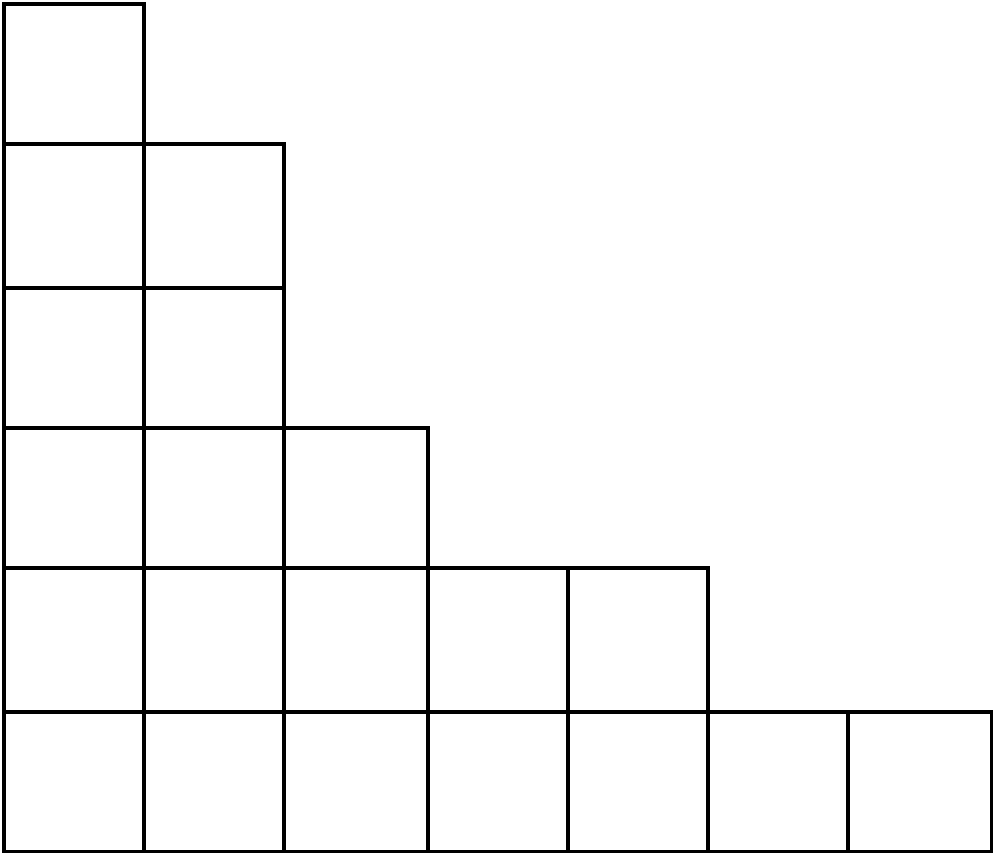
\includegraphics[width=0.5\linewidth]{Images/Figure17.png}
    \caption{The Ferrer's diagram for $7+5+3+2+2+1$}
\end{figure}
It is clear that height of the Ferrer's diagram corresponds to the number of parts in the partition and that the width corresponds to the size of the largest part in the partition. To this end, consider the following result. 
\begin{theorem}
The number of partitions of $n$ into atmost $i$ parts, each of which is atmost $j$ is the same as the number of partitions of $n$ into atmost $j$ parts, each of which is atmost $i$. 
\end{theorem}
\begin{proof}
Let $\pi$ a partition of $n$ into at most $i$ parts each of which is at most $j$. The Ferrer's diagram corresponding to $\pi$ now has height at mmost $i$ and width at most $j$. Flipping the said diagram about its main diagonal results in a diagram that has height at most $j$ and width at most $i$. Finally, the partition corresponding to this flipped diagram (called the conjugate partition) is a partition of $n$ into atmost $j$ parts, each of which is atmost $i$. 
\end{proof}
\begin{figure}[H]
    \centering
    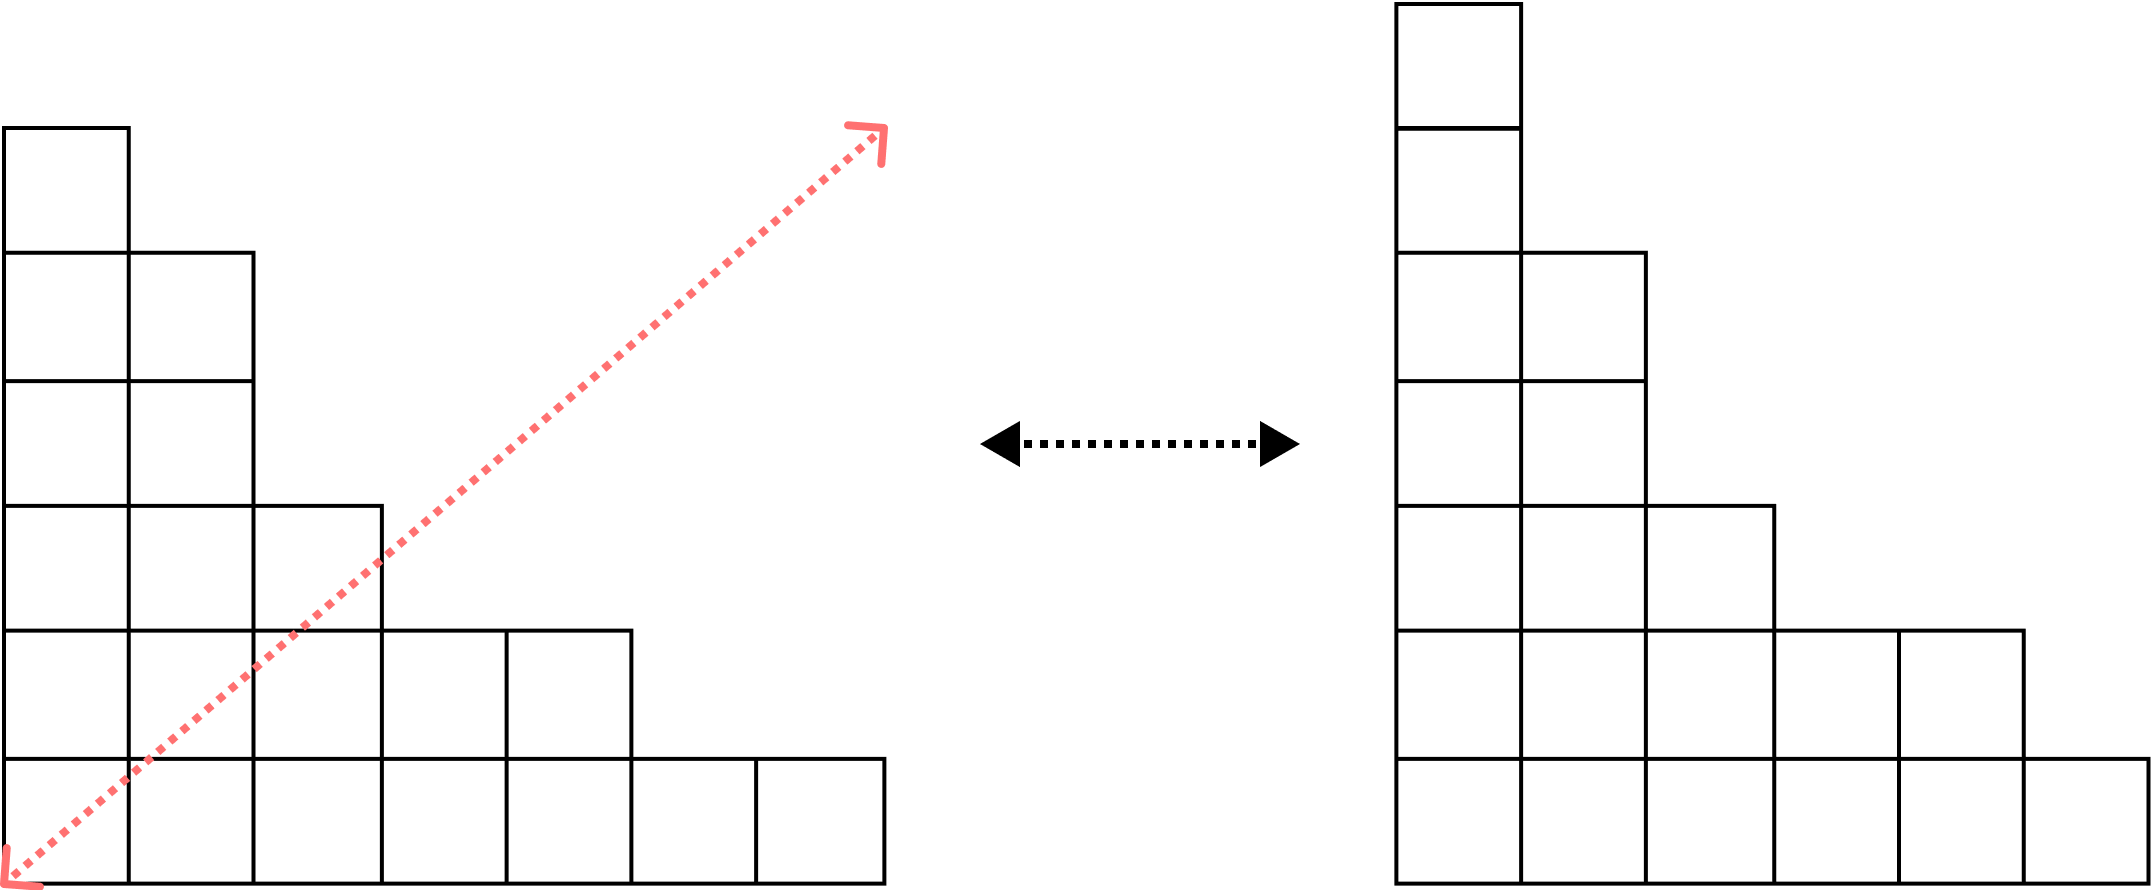
\includegraphics[width=0.8\linewidth]{Images/Figure18.png}
    \caption{An example of the conjugate of $7+5+3+2+2+1$}
\end{figure}
Another useful pictorial construct is that of a Durfee square. We define the said square to be the largest one which can fit in the Ferrer’s diagram corresponding to a partition.
\begin{figure}[H]
    \centering
    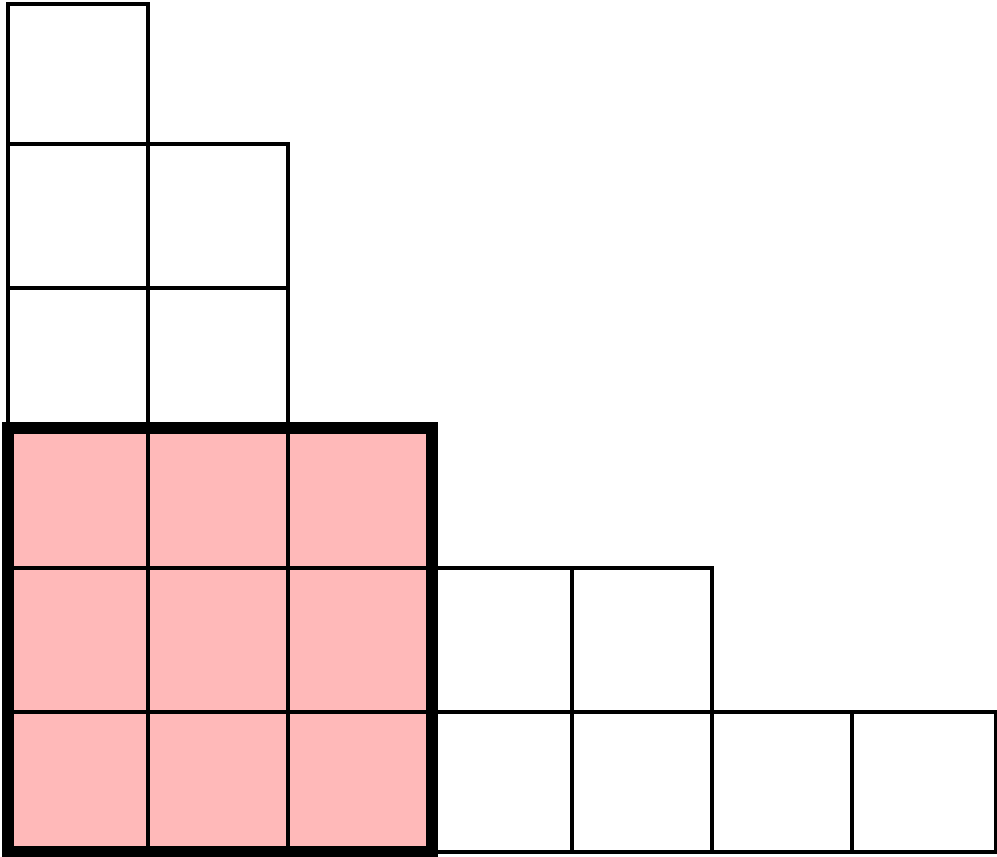
\includegraphics[width=0.5\linewidth]{Images/Figure19.png}
    \caption{The Durfee square of order $3$ in the partition $7+5+3+2+2+1$}
    \label{DurfeeExample}
\end{figure}
(Keeping in mind \cref{DurfeeExample}) notice how
\begin{enumerate}
    \item Every non-empty partition has a Durfee square of order $k$ (if nothing, you always have the Durfee square of order $k=1$).
    \item Partitions corresponding to the triangle above the Durfee square are the ones where each part is at most $k$.
    \item Partitions corresponding to the triangle below the Durfee square are the ones where the number of parts is at most $k$. 
\end{enumerate}
With these three observations at hand, an identity presents itself almost immediately. Namely,
\begin{claim}[Jacobi's Identity]
    \[
    \prod_{i=1}^{\infty}\dfrac{1}{1-q^i} = \sum_{i=0}^{\infty}\dfrac{q^{i^2}}{(1-q)^2(1-q^2)^2\cdots(1-q^i)^2}
    \]
    \label{c:DurfeeId1}
\end{claim}
Next, we state a remarkable result first proved by Euler in the year 1785.
\begin{theorem}[Euler's Pentagonal Number Theorem]
\begin{align*}
\prod_{i=1}^{\infty}(1-q^i) &= \sum_{k=-\infty}^{\infty}(-1)^k q^{\dfrac{k(3k-1)}{2}} \\
&= 1+\sum_{k=1}^{\infty}(-1)^kq^{\dfrac{k(3k-1)}{2}}+\sum_{k=-\infty}^{-1}(-1)^kq^{\dfrac{k(3k-1)}{2}} \\
&= 1+\sum_{k=1}^{\infty}(-1)^kq^{\dfrac{k(3k-1)}{2}}+\sum_{k=1}^{\infty}(-1)^kq^{\dfrac{k(3k+1)}{2}} \\
&= 1+\sum_{k=1}^{\infty}(-1)^k \left(q^{\dfrac{k(3k-1)}{2}}+q^{\dfrac{k(3k+1)}{2}}\right) \\
\end{align*}
\label{t:EPT}
\end{theorem}
We are interested in starting three different proofs of the theorem. Before moving on to them, it would help to understand what pentagonal numbers are. Simply put, these are numbers of the form $n(3n-1)/2$. Why they are called pentagonal is clear from the following figure.
\begin{figure}[H]
    \centering
    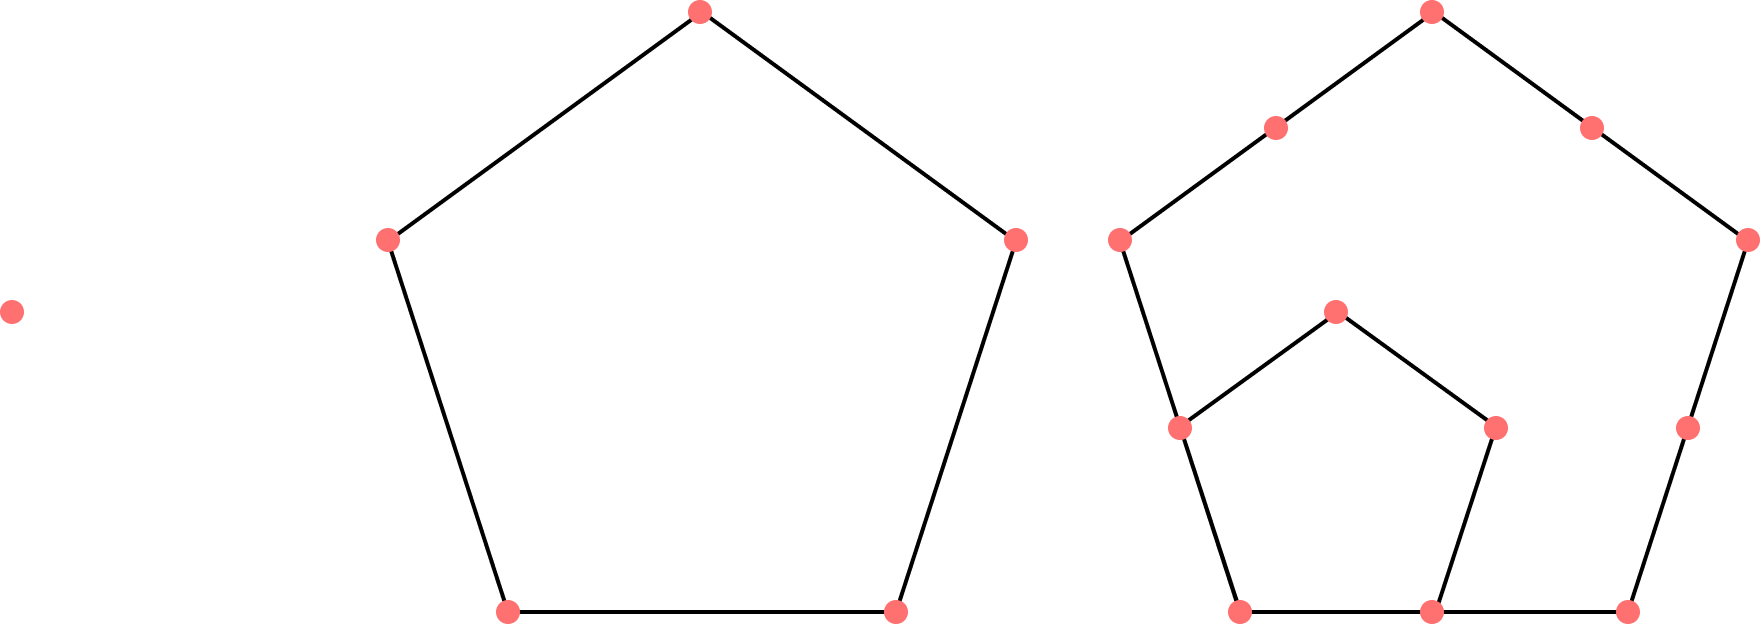
\includegraphics[width=0.8\linewidth]{Images/Figure20.png}
    \caption{Counting the number of vertices (marked in red) at each iteration gives the sequence of pentagonal numbers, i.e, $1,5,12,\ldots$}
    \label{f:PNT}
\end{figure}
Notice how the vertices (marked in red) in \cref{f:PNT} admit a natural partition and hence a Ferrer's diagram. 
\begin{figure}[H]
    \centering
    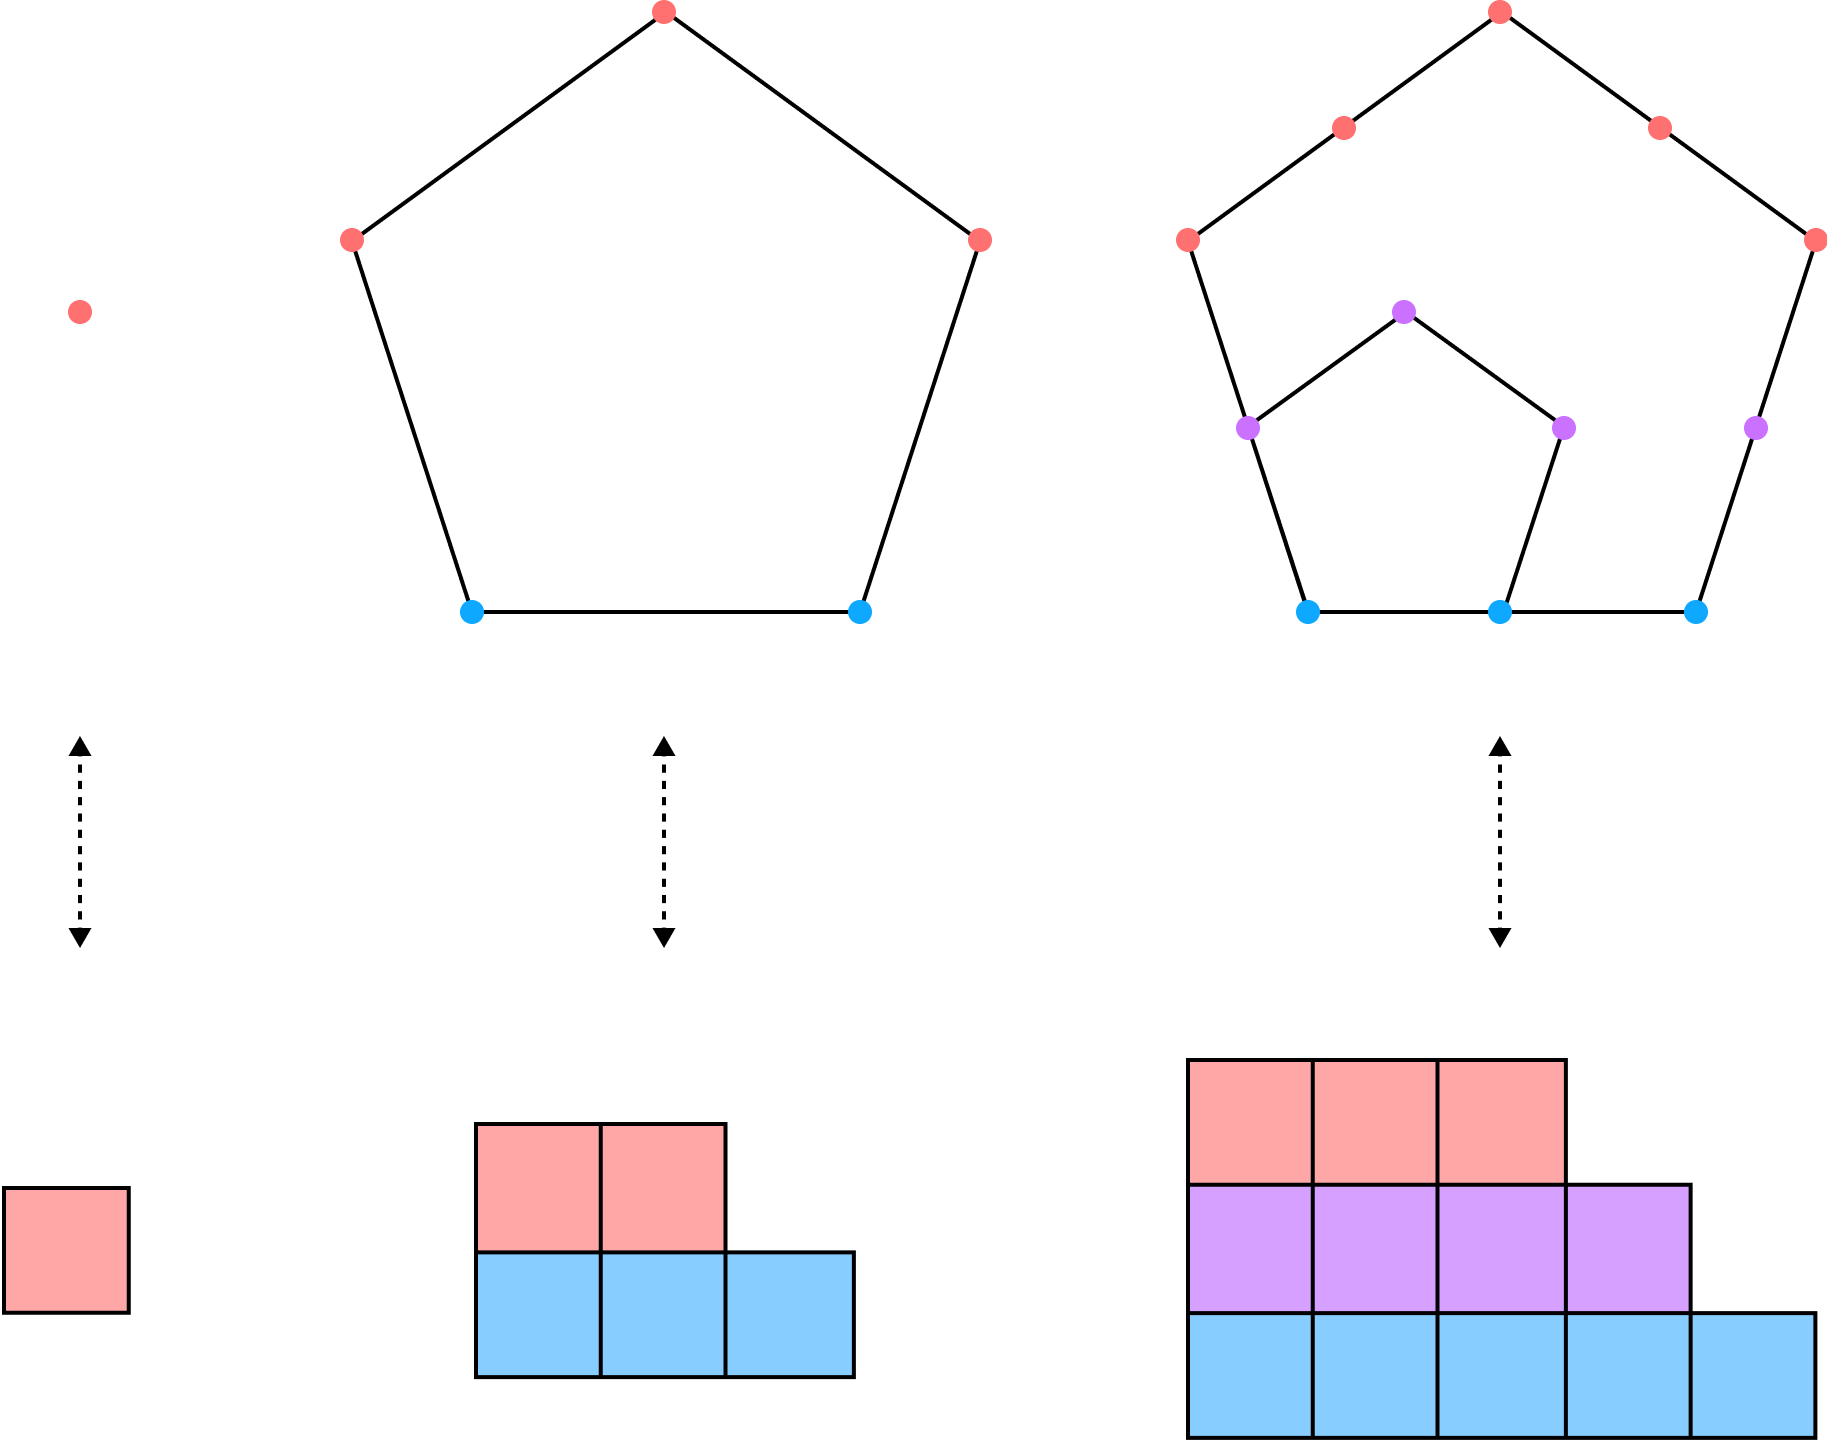
\includegraphics[width=0.8\linewidth]{Images/Figure21.png}
    \caption{The first $3$ pentagonal numbers and the natural partitions they admit, i.e, $1=1, 5=3+2$, and $12=5+4+3$.}
\end{figure}
These partitions of pentagonal numbers we have obtained are partitions into distinct parts. To this end, we will try and set up a bijection between partitions of $n$ into an odd number of distinct parts and the partitions of $n$ into an even number of distinct parts. Consider the following auxiliary claim.
\begin{claim}
Let $p_{e}(n)$ and $p_{o}(n)$ denote the number of partitions of $n$ into an even and odd number of distinct parts respectively. Then
\[
p_{e}(n)-p_{o}(n) = \begin{cases}
    (-1)^m \quad &\text{if } n = \dfrac{m(3m\pm 1)}{2} \\
    0 \quad &\text{otherwise}
\end{cases}
\]
\label{t:EPT_Aux}
\end{claim}
\begin{proof}
Let $\lambda$ be a partition of $n$. Let $s(\lambda)$ and $\sigma(\lambda)$ denote the smallest part of $\lambda$ and the part obtained by considering elements on the rightmost diagonal respectively. If $s(\lambda)\leq \sigma(\lambda)$, we add one to each of the $s(\lambda)$ largest parts of $\lambda$ and we delete the smallest part. Consider the following example for instance.
\begin{figure}[H]
    \centering
    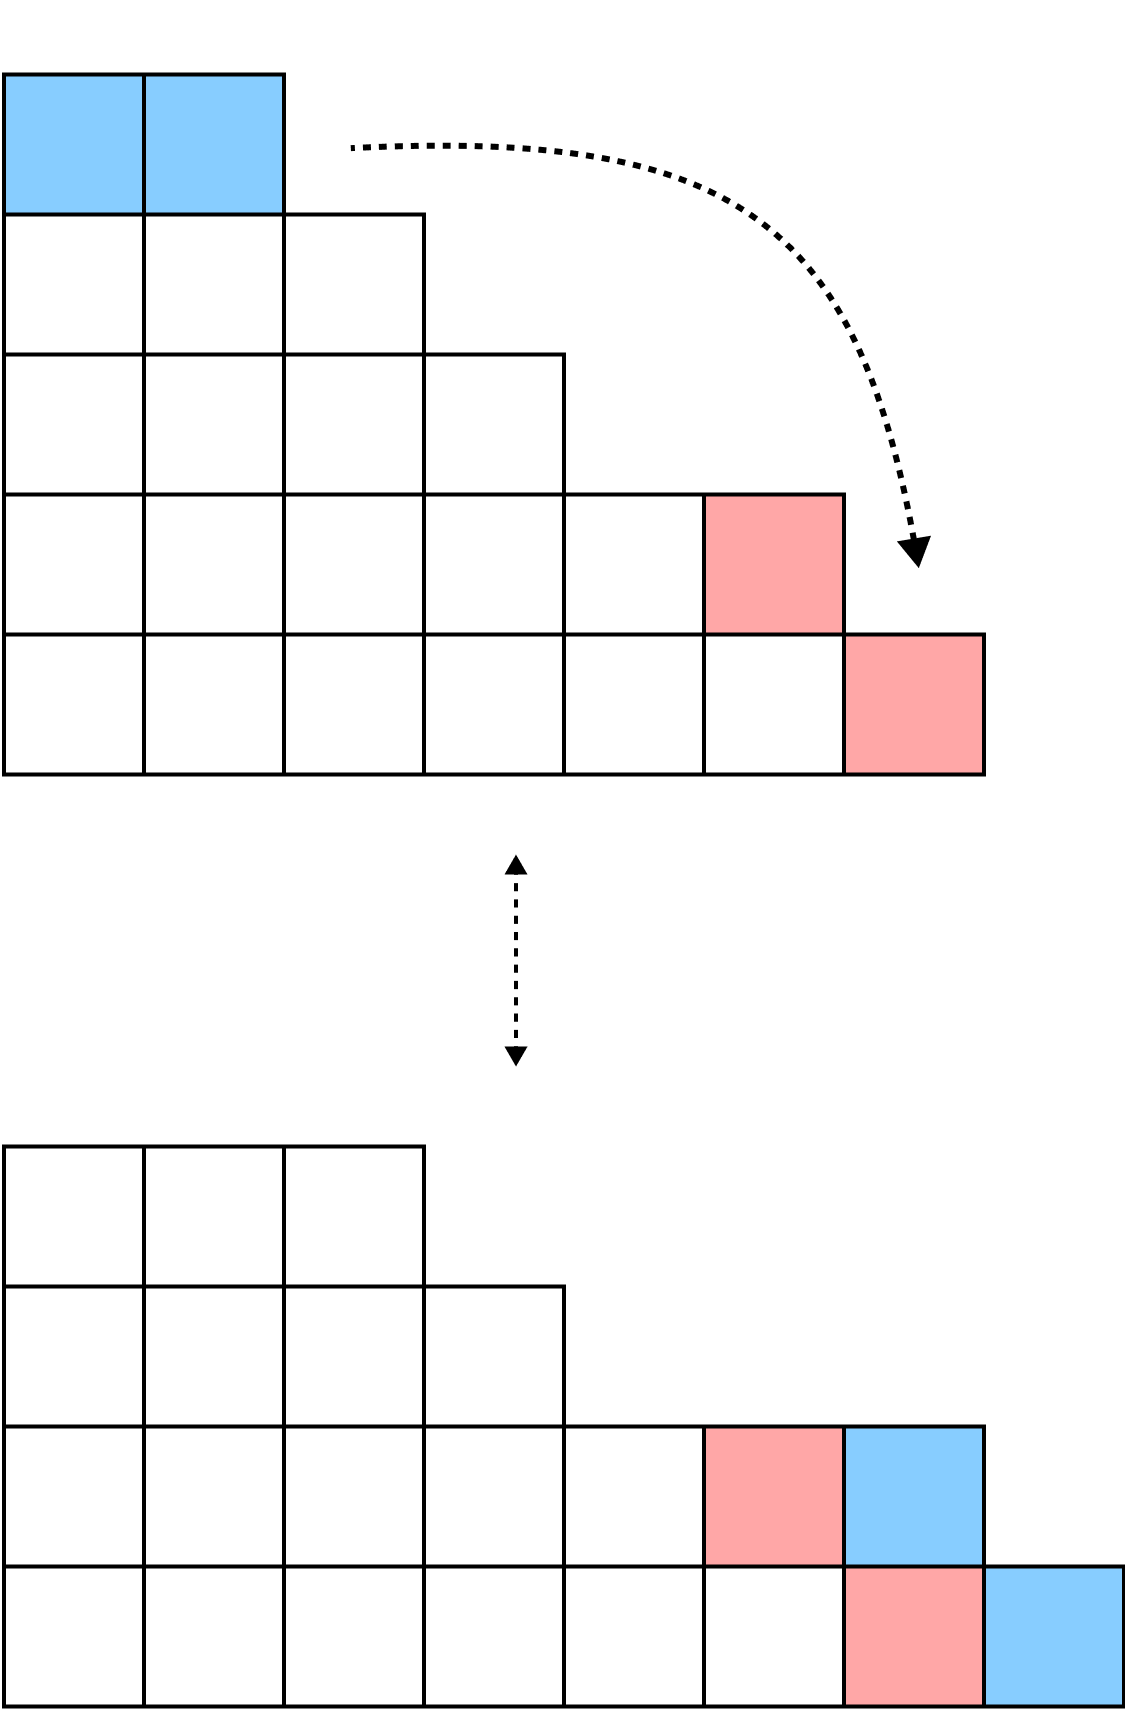
\includegraphics[width=0.4\linewidth]{Images/Figure24.png}
    \caption{The partition $\lambda=7+6+4+3+2$ with $s(\lambda)=2$ (marked blue) and $\sigma(\lambda)=2$ (marked red) admits the partition $\lambda'=8+7+4+3$.}
\end{figure}
On the other hand, if $s(\lambda)>\sigma(\lambda)$ then we subtract one from each of the $\sigma(\lambda)$ largest parts of $\lambda$ and insert a new smallest part of size $\sigma(\lambda)$. Consider the following example for instance.
\begin{figure}[H]
    \centering
    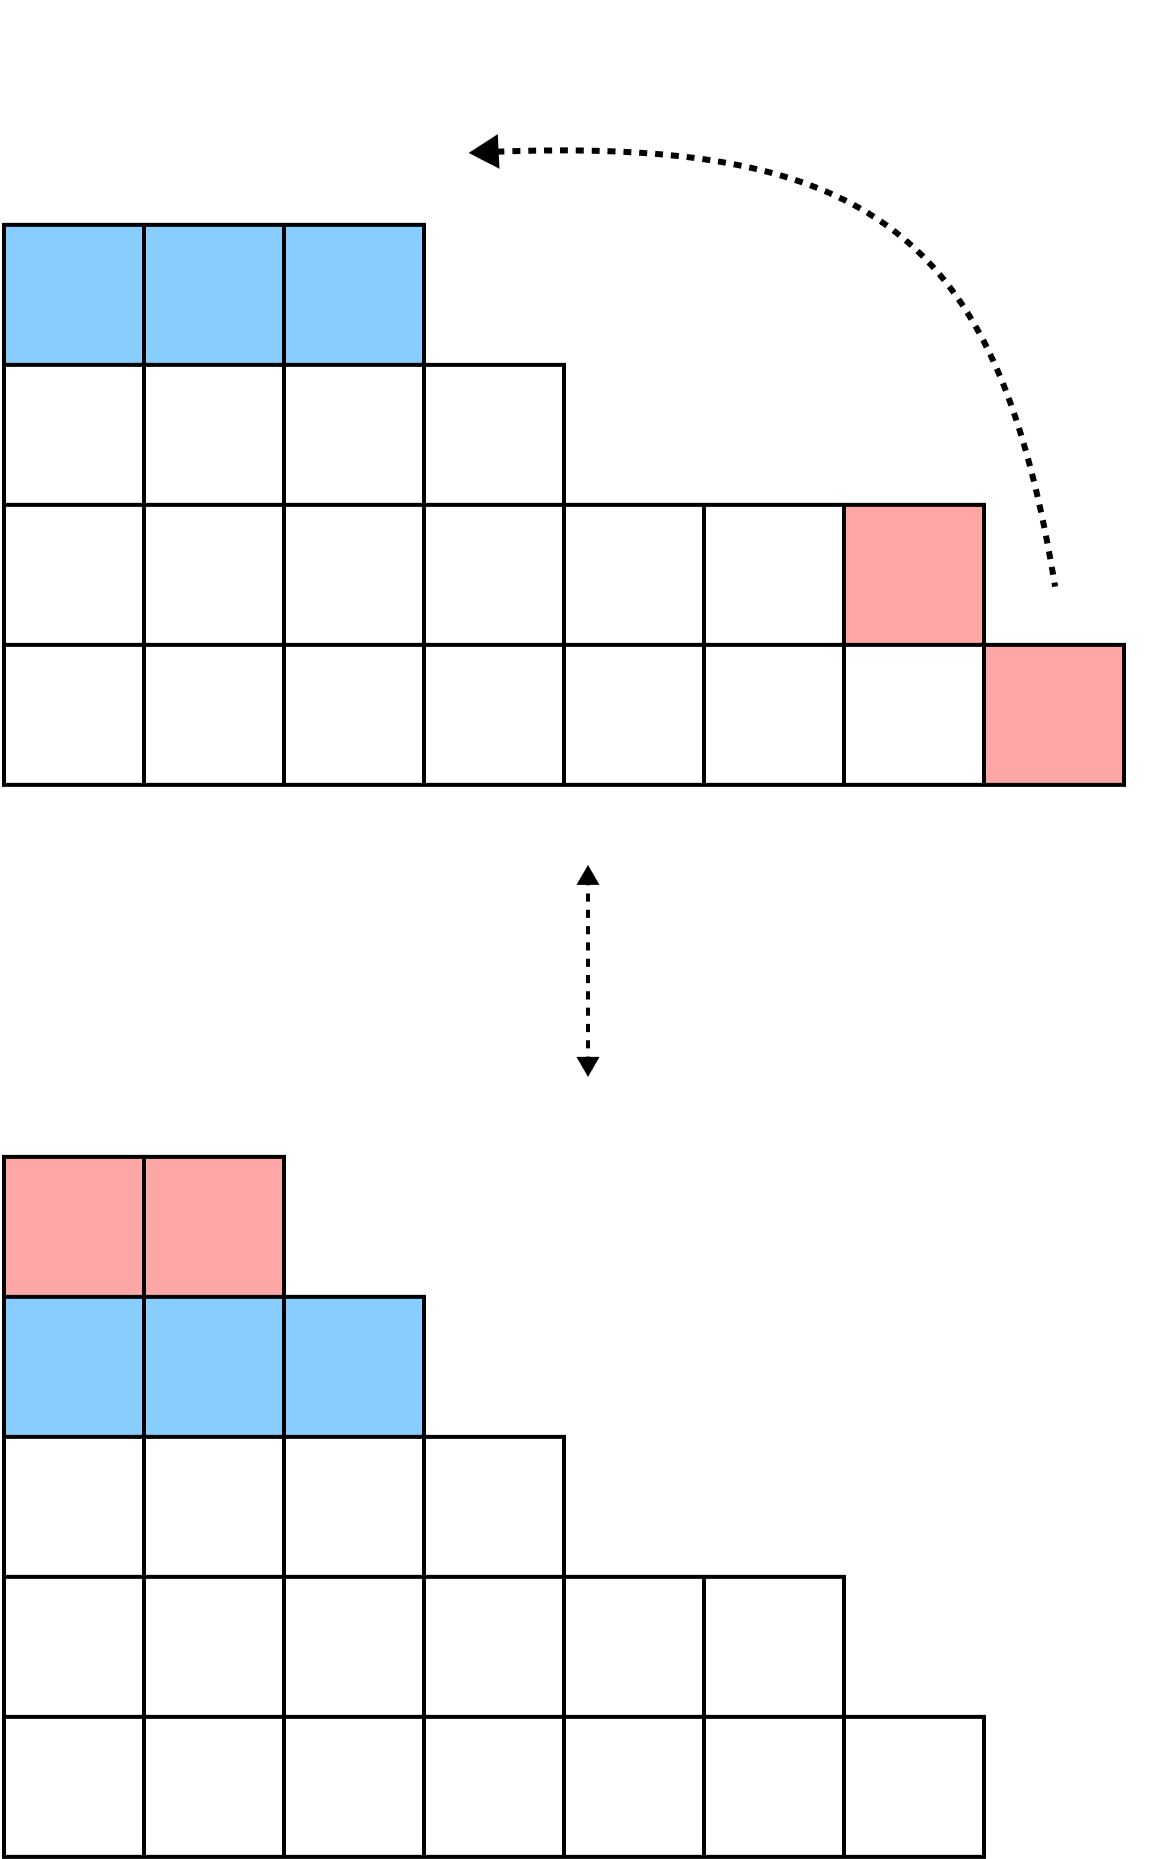
\includegraphics[width=0.4\linewidth]{Images/Figure25.png}
    \caption{The partition $\lambda=8+7+4+3$ with $s(\lambda)=3$ (marked blue) and $\sigma(\lambda)=2$ (marked red) admits the partition $\lambda'=7+6+4+3+2$.}
\end{figure}
In summary, our map changes the parity of the number of parts of the partition, and noting that exactly one case applies to any partition, it is clear why our map is a bijection. However, we are not done yet! Our map fails in two cases. One, where $s(\lambda)=m+1$ is exactly one more than $\sigma(\lambda)=m$, i.e, the case where the number being partitioned is \[
(m+1)+(m+2)+\cdots+2m = m(3m+1)/2.
\]
Two, where $s(\lambda)=\sigma(\lambda)$, i.e, the case where the number being partitioned is \[
m+(m+1)+\cdots+(2m-1) = m(3m-1)/2.
\]
This completes the proof. 
\end{proof}
Now, \cref{t:EPT} follows as a direct consequence of \cref{t:EPT_Aux}. 
\par
To see the usefulness of \cref{t:EPT} consider the following remark.
\begin{remark}
Putting \cref{t:EPT} and \cref{c:2.1P} together gives us \[
\left(\sum_{n\geq 0}p(n)q^n\right)\left(\prod_{i\geq 1}(1-q^i)\right) = 1.
\] A recurrence of sorts presents itself. Namely,
\[
p(n) = p(n-1)+p(n-2)-p(n-5)-p(n-7)+p(n-12)+p(n-15)+\cdots. 
\] The reason this recurrence is useful is two-pronged. One, the sum on the right is not infinite because $p(k)=0$ for all choices of $k<0$. Two, to compute $p(n)$ we need not compute $p(n-i)$ for all choices of $1\leq i\leq n-1$.
\end{remark}
Next, we present a result known as Jacobi's triple product identity. Interestingly, this identity is easier to prove than Euler's pentagonal number theorem. Not only that, but, Euler's theorem emerges as a corollary of Jacobi's identity. Before stating the identity, we introduce some useful notation. For formal variables $x,q$ and a natural number $n>0$ we define
\[
(x;q)_n := (1-x)(1-xq)(1-xq^2)\cdots(1-xq^{n-1}) = \prod_{i=0}^{n-1}(1-xq^i).
\]
The symbol $(x;q)_n$ is referred to as the $q$-shifted factorial. We extend our notation to allow for $n$ to be $\infty$ by defining
\[
(x;q)_\infty := \lim_{n\to \infty}\left(\prod_{i=0}^{n-1}(1-xq^i)\right) = \prod_{i=0}^{\infty}(1-xq^i) = (1-x)(1-xq)(1-xq^2)\cdots.
\]
It follows (by setting $x$ to $q$) that
\begin{align*}
    &(q;q)_n = (1-q)(1-q^2)\cdots(1-q^n) = \prod_{i\geq 1}^n (1-q^i)\\
    &(q;q)_\infty = (1-q)(1-q^2)\cdots = \prod_{i\geq 1}(1-q^i)
\end{align*}
\raggedbottom
In the spirit of getting comfortable with the newly introduced notation it is a good exercise to verify the following re-statements of the claims we have made so far;
\begin{align*}
    &\sum_{n \geq 0} p(n) q^n = \dfrac{1}{(q;q)_\infty} \quad (\text{Refer to } \cref{c:2.1P}) \\
    &\sum_{n \geq 0} p_D(n) q^n = (-q;q)_\infty \quad (\text{Refer to } \cref{t:Euler'sGem}) \\
    &\sum_{n \geq 0} \dfrac{q^{n^2}}{(q;q)_n^2} =\dfrac{1}{(q;q)_\infty}\quad (\text{Refer to } \cref{c:DurfeeId1})
\end{align*}
To see the usefulness of our notation, we introduce ourselves to a bi-variate generating function. Consider the expansion of $1/(xq;q)_\infty$ in which the coefficient of $x^k$ is $1/(q;q)_k$. More succinctly put we get;
\begin{claim}
\[\sum_{n\geq 0}^\infty\dfrac{x^n}{(q;q)_n} = \dfrac{1}{(x;q)_\infty}.\]
\end{claim}
A more natural interpretation of the identity comes from setting $x\to xq$ to arrive at
\[
\sum_{n\geq 0}^\infty \dfrac{x^kq^k}{(q;q)_k} = \dfrac{1}{(xq;q)_\infty}.
\]
Now the coefficient of $x^k$ is the generating function for partitions with exactly $k$ parts. 
\par
Now we are at a stage to introduce ourselves to Jacobi's triple product identity.
\begin{theorem}[Jacobi Triple Product]
For $|q|<1$ and $z\neq 0$ we have 
\[
\sum_{n=-\infty}^{\infty}q^{n^2}z^n = (q^2;q^2)_\infty (-q/z;q^2)_\infty (-zq;q^2)_\infty
\]
\end{theorem}
Before giving a proof of the identity, we remark that by setting $q\to q^{3/2}$ and $z\to -\sqrt{q}$ we retrieve Euler's pentagonal number theorem back. 
\begin{proof}
\textcolor{red}{[Note to scribe: Finish the proof(s)!]}
\end{proof}
Next, we turn our attention to an identity due to Sylvester. One reason why this identity is important is because Euler's pentagonal theorem presents itself as a corollary of Sylvester's identity. 
\begin{theorem}[Sylvester's Identity]
\[
		\left( -xq;q \right)_{\infty} = 1+\sum_{k=1}^{\infty}x^kq^{\frac{k\left( 3k-1 \right) }{2}}\frac{\left( -xq;q \right)_{k-1}}{\left( q;q \right)_{k}}\left( 1+xq^{2k}\right)  
\]
\end{theorem}
Before giving a proof of the identity, we remark that by setting 
$x\to -1$ we retrieve Euler's pentagonal number theorem back. Next, we make a few observations about the Ferrer's diagram corresponding to a partition which has distinct parts which will turn out to be important while writing a combinatorial proof of Sylvester's Identity.   
\begin{figure}
    \centering
    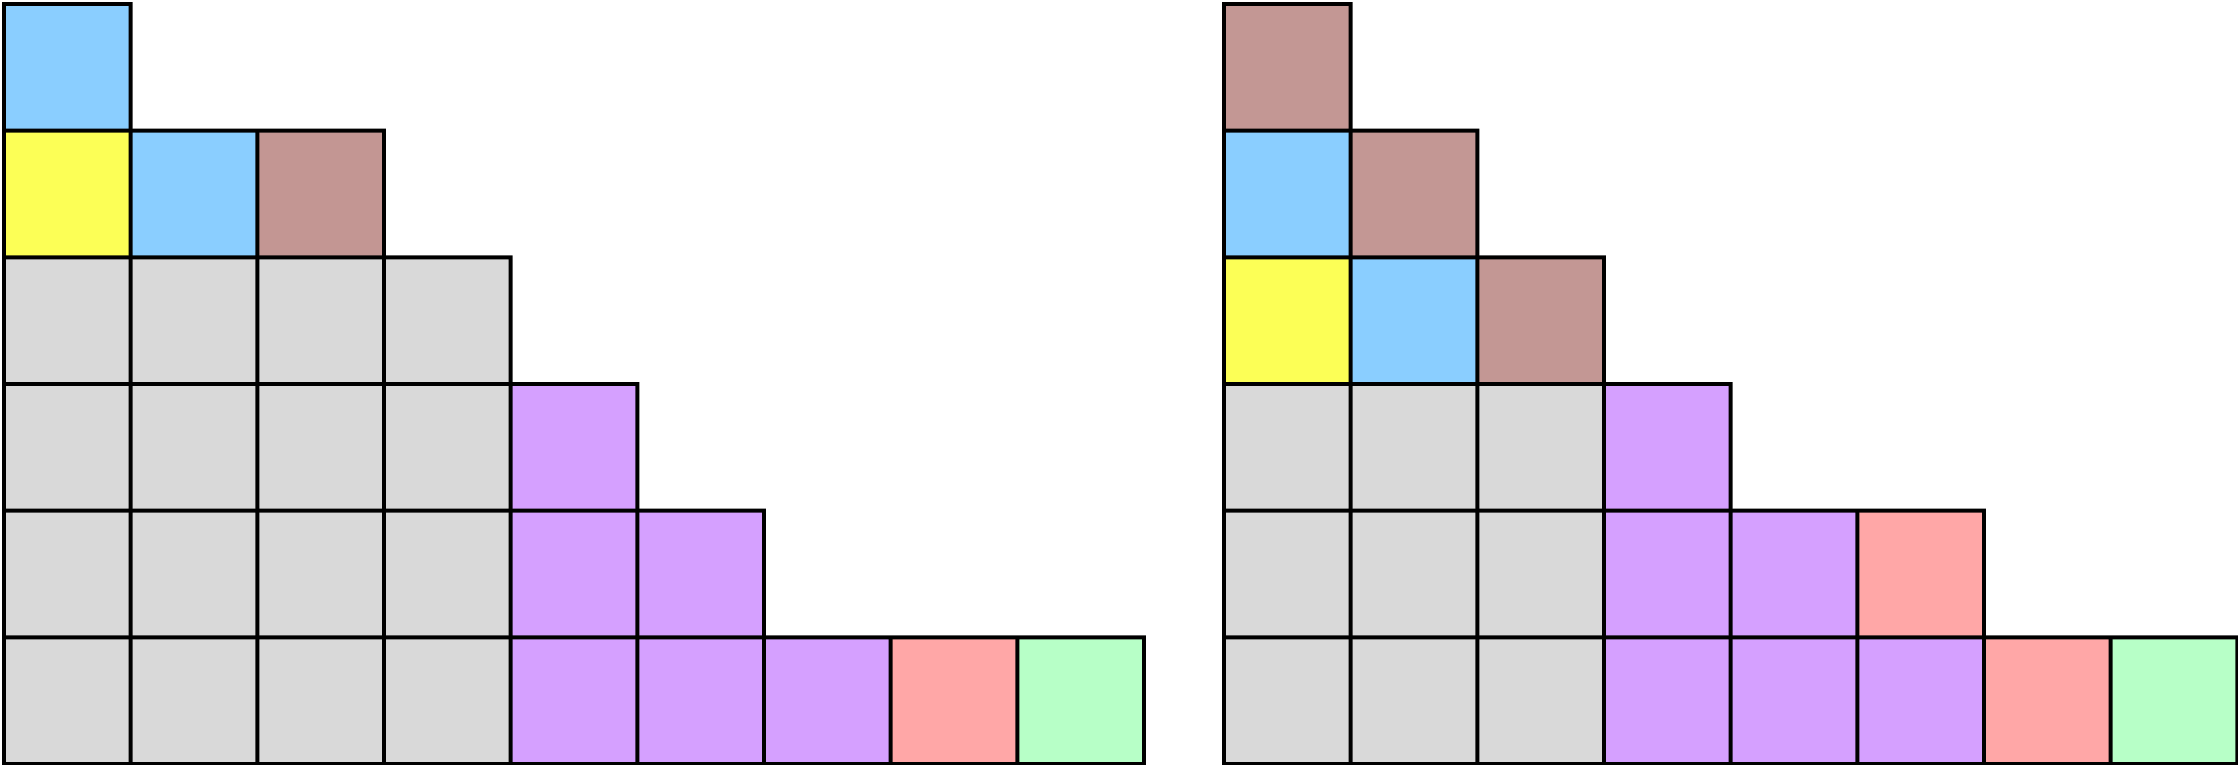
\includegraphics[width=0.8\linewidth]{Images/Figure26.png}
    \caption{Franklin Triangles}
    \label{f:FranklinTsF}
\end{figure}
Refer to \cref{f:FranklinTsF} and notice how if the said diagram has a Durfee square (colored grey) of order $k$, then to the right of this square, there must be an isoceles triangle (colored purple, and called the \textbf{Franklin} triangle) of length either $k$, or $k-1$, depending on where the Durfee square ends. In the case where the Franklin triangle is of order $k-1$;   
\begin{enumerate}
			\item The Durfee square and the Franklin triangle correspond to a unique partition of $k^2+\binom{k}{2}$
			\item The pieces to the right of the Franklin triangle, when counted diagonally, correspond to partitions where each part is atmost $k-1$.
			\item The pieces below the Franklin triangle, when counted diagonally, correspond to partitions into atmost $k-1$ parts.
\end{enumerate}
Similarly, in the case where the Franklin triangle is of order $k$;
\begin{enumerate}
			 \item The Durfee square and the Franklin triangle correspond to a unique partition of $k^2+\binom{k+1}{2}$
			 \item The pieces to the right of the Franklin triangle, when counted diagonally, correspond to partitions where each part is atmost $k$.
			 \item The pieces below the Franklin triangle, when counted diagonally, correspond to partitions into atmost $k$ parts.
		\end{enumerate}
\begin{proof}
    We know that the coefficient of $x^iq^j$ in $\left( -xq;q \right)_{\infty}$ is the number of partitions of $j$ into exactly $i$ parts each of which is distinct. But every such partition has a Durfee square of order atleast $k=1$, and a Franklin triangle of order either $k-1$, or $k$ in it's Ferrer's diagram. From the observations made above, we get
 \begin{align*}
	 \left( -xq;q \right)_{\infty} &= \underbrace{\sum_{k=1}^{\infty} x^kq^{k^2+\binom{k}{2}}\frac{\left( -xq;q \right)_{k-1}}{\left( q;q \right)_{k-1}}}_{\text{Order of Franklin triangle: } k-1} + \underbrace{\sum_{k=0}^{\infty} x^kq^{k^2+\binom{k+1}{2}} \frac{\left( -xq;k \right)_{k}}{\left( q;q \right)_{k}}}_{\text{Order of Franklin triangle: } k} \\
				       &= \sum_{k=1}^{\infty} x^k q^{k^2+\binom{k}{2}} \frac{\left( -xq;q \right)_{k-1}}{\left( q;q \right)_{k-1}} + 1 + \sum_{k=1}^{\infty}x^kq^{k^2+k+\binom{k}{2}}\frac{\left( -xq;q \right)_{k-1}}{\left( q;q \right)_{k-1}}\frac{\left( 1+xq^k \right)}{1-q^k} \\
				       &= 1+\sum_{k=1}^{\infty} x^kq^{k^2+\binom{k}{2}}\frac{\left( -xq;q \right)_{k-1}}{\left( q;q \right)_{k-1}}\left( 1+\frac{q^k\left( 1+xq^k \right)}{\left( 1-q^k \right) } \right)  \\
				       &= 1+\sum_{k=1}^{\infty} x^kq^{k^2+\binom{k}{2}}\frac{\left( -xq;q \right)_{k-1}}{\left( q;q \right)_{k-1}\left( 1-q^k \right)}\left( 1+xq^{2k} \right) \\
				       &= 1+\sum_{k=1}^{\infty} x^kq^{k^2+\binom{k}{2}}\frac{\left( -xq;q \right)_{k-1}}{\left( q;q \right)_{k}}\left( 1+xq^{2k} \right)
\end{align*}
\end{proof}
Next, we give an analytic proof of the same identity. 
\begin{proof}
Notice how 
\begin{align*}
    f(x):&= 1+\sum_{k=1}^{\infty}x^kq^{k(3k-1)/2}\dfrac{(-xq;q)_{k-1}}{(q;q)_k}(1+xq^{2k}) \\
    &= 1+\sum_{k=1}^{\infty}x^kq^{k(3k-1)/2}\dfrac{(-xq;q)_{k-1}}{(q;q)_k}\left((1-q^k)+q^k(1+xq^k)\right) \\
    &= 1+\sum_{k=1}^{\infty}x^kq^{k(3k-1)/2}\dfrac{(-xq;q)_{k-1}}{(q;q)_{k-1}}+\sum_{k=1}^{\infty}x^kq^{k(3k+1)/2}\dfrac{(-xq;q)_k}{(q;q)_k} \\
    &= \sum_{k=0}^{\infty}x^kq^{k(3k+1)/2}\dfrac{(-xq;q)_k}{(q;q)_k}+\sum_{k=0}^{\infty}x^{k+1}q^{(k+1)(3k+2)/2}\dfrac{(-xq;q)_k}{(q;q)_k} \\
    &= \sum_{k=0}^{\infty}x^k q^{k(3k+1)/2}q^{k(3k+1)/2}\dfrac{(-xq;q)_k}{(q;q)_k}(1+xq^{2k+1}).
\end{align*}
Our observation allows us to conclude that
\[
f(x) = (1+xq)\left(
1+\sum_{k=1}^{\infty}x^kq^{k(3k+1)/2}\dfrac{(-xq^2;q)_{k-1}}{(q;q)_k}(1+xq^{2k+1}).
\right)
\]
More succinctly, $f(x)=(1+xq)f(xq)$, iterating which we get $f(x)=(-xq;q)_\infty$ as required. 
\end{proof}
We conclude this section on integer partitions by discovering a Rogers-Ramanujan identities. Namely, 
\begin{align*}
    &\sum_{n=0}^{\infty}\dfrac{q^{n^2}}{(q;q)_n} = \dfrac{1}{(q;q^5)_\infty(q^4;q^5)_\infty}, \\
    &\sum_{n=0}^{\infty}\dfrac{q^{n^2+n}}{(q;q)_n} = \dfrac{1}{(q^2;q^5)_\infty (q^3;q^5)_\infty}.
\end{align*}
Doing so requires some familiarity with continued fractions. As an example consider the fraction
\[
C = 1+\dfrac{1}{1+\dfrac{1}{1+\dfrac{1}{1+\ddots}}}.
\]
Truncating the fraction at various depths gives us a sequence of what are called convergents. Observing the convergents of $C$, \[
\dfrac{1}{1},\dfrac{2}{1},\dfrac{3}{2},\dfrac{5}{3},\dfrac{8}{5},\cdots
\]
makes it clear that the $n$-th convergent is given by $f_n/f_{n-1}$ where $f_n$ denote the $n$-th Fibonacci number. Next, we give a two-parameter generalization of $C$, called the Rogers-Ramanujan continued fraction, in the variables $z$ and $q$.
\[
C(z,q) = 1+\dfrac{zq}{1+\dfrac{zq^2}{1+\dfrac{zq^3}{1+\ddots}}}.
\]
Observing the convergents of $C(z,q)$,
\[
1,1+zq,(1+zq+zq^2)/(1+zq^2),(1+zq+zq^2+zq^3+z^2q^4)/(1+zq^2+zq^3), \cdots,
\]
makes it clear that the $n$-th convergent is of the form 
\begin{align*}
H_n(z,q)/H_{n-1}(zq,q) = 1+\dfrac{zqH_{n-2}(zq^2,q)}{H_{n-1}(zq,q)}.
\end{align*}
Additionally, it is also not difficult to verify that $C(z,q)=1+zq/C(zq,q)$. Putting both of our observations together, it is seems logical to assume that $C(z,q)$ must be of the form $H(z,q)/H(zq,q) = 1+zqH(z^q,q)/H(zq,q)$. This gives the recurrence $H(z,q)=H(zq,q)+zqH(z^2q,q)$ which is solve using the method of generating functions to see that if $H(z,q)=\sum_{k=0}^\infty a_kz^k$, then
\begin{align*}
& a_k = a_kq^k + a_{k-1}q^{2k-1} \\
&\implies a_k = (q^{2k-1}/1-q^k)a_{k-1} \\
&\implies a_k = (q^{k^2}/(q;q)_k)a_0.
\end{align*}
Since $a_0 = 1$, it follows that \[
H(z,q) = \sum_{k-0}^{\infty}\dfrac{q^{k^2}}{(q;q)_k}z^k.
\]
Finally, since $C(1,q)=H(1,q)/H(q,q)$ we get the two Rogers-Ramanujan identities. 
\par
Notice how $1/(q;q^5)_\infty(q^4;q^5)_\infty$ and $1/(q^2;q^5)_\infty(q^3;q^5)_\infty$ are the generating functions for partitions into parts which are congruent to $1,4\mod{5}$ and $2,3\mod{5}$ respectively. Additionally, $q^{n^2}/(q;q)_n$ is the generating functions for partitions with exactly $n$ parts having a difference of atleast $2$. Finally, $q^{n^2+n}/(q;q)_n$ is the same generating function but the smallest part is not allowed to be less than $2$. Putting all these observations together, we draw the following combinatorial interpretations. One, the number of partitions of \( n \) with \( k \) parts, where the smallest part is at least \( k \), is equal to the number of partitions of \( n \) in which each part is congruent to either \( 1 \) or \( 4 \) modulo \( 5 \). Two, the number of partitions of \( n \) with \( k \) parts, where the smallest part is at least \( k+1 \), is equal to the number of partitions of \( n \) in which each part is congruent to either \( 2 \) or \( 3 \) modulo \( 5 \).
\endinput
